%------------------------------------------------------------
\title[02 - 函数Ⅱ]
{02 - 函数Ⅱ}

\subtitle{C++ 程序设计进阶}

\author[Beiyu Li]
{Beiyu Li\\
\texttt{<sysulby@gmail.com>}}

% \institute[SOJ]
% {Sicily Online Judge}

\date[\today]
{\number\year 年 \number\month 月 \number\day 日}
%------------------------------------------------------------


\begin{document}

\author[sysulby]
{SOJ 信息学竞赛教练组}

\begin{frame}
    \titlepage
\end{frame}
\setcounter{framenumber}{0} % 标题页不编号

\section{复习回顾}

%------------------------------------------------------------

%------------------------------------------------------------
\begin{frame}[fragile]
    \frametitle{函数的定义}

    \begin{itemize}[<+->]
        \item 函数的定义形式如下:
        \lstinputlisting[basicstyle=\ttfamily\scriptsize,language=C++,name=functionStructure2]{ch13/functionStructure2.cc}
        \item 需要写在 \textbf{\lstinline|main| 函数外面}
        \item 确定函数的\textbf{功能},把功能的实现写在函数体中
    \end{itemize}
\end{frame}
%------------------------------------------------------------

%------------------------------------------------------------
\begin{frame}[fragile]
    \frametitle{函数的调用}

    \only<1-3>{
        \begin{columns}
            \column{.45\textwidth}
            \begin{itemize}
                \item<1-> 形式参数、实际参数
                \item<4-> 1
                \begin{itemize}
                    \item<5-> 1
                    \item<6-> 1
                    \item<7-> 1
                    \item<8-> 1
                \end{itemize}
            \end{itemize}
        
            \column{.55\textwidth}
            \lstinputlisting[basicstyle=\ttfamily\scriptsize,language=C++,name=printNHelloWorld]{ch13/printNHelloWorld.cc}
            \begin{tikzpicture}[remember picture,overlay]
                \uncover<3->{\redbox{printNHelloWorld}{12}{9}{12}{9} node[right,xshift=.2cm]{实际参数};}
                \uncover<2->{\redbox{printNHelloWorld}{5}{12}{5}{16} node[right,xshift=.2cm,yshift=.5cm]{形式参数};}
            \end{tikzpicture}
        \end{columns}
    }

    \only<4-9>{
        \begin{itemize}
            \item<4-> 形式参数、实际参数
            \item<4-> 调用函数
            \begin{itemize}
                \item<5-> \lstinline|函数名(实参1, 实参2, …);|
                \item<6-> 无参数时也要保留小括号
                \item<7-> 注意参数顺序要对应
                \item<8-> 求 $2$ 的 $10$ 次方:\only<8>{\lstinline|pow(10,2)|} \uncover<9>{\redout{\lstinline|pow(10,2)|} \textcolor{red}{\lstinline|pow(2,10)|}}
            \end{itemize}
        \end{itemize}
    }

    \only<10->{
        \begin{itemize}[<+->]
            \item 调用无返回值的函数
            
            \begin{itemize}
                \item 直接调用
            \end{itemize}

            \item 调用有返回值的函数
            
            \begin{itemize}
                \item 处理返回的结果,直接使用或存储后使用
            \end{itemize}

        \end{itemize}
    }
    
\end{frame}
%------------------------------------------------------------


\section{模块化编程}

%------------------------------------------------------------
\begin{frame}[fragile]
    \frametitle{函数的使用场景}

    \alt<2-6>{
        \begin{itemize}
            \item<2-> 多次使用相同功能
            
            \begin{itemize}
                \item<3-> 五边形面积
            \end{itemize}

            \item<4-> 复杂的逻辑嵌套
            
            \begin{itemize}
                \item<5-> 质数判断
            \end{itemize}

        \end{itemize}
    }{
        \begin{block}{}
            \vspace{.5cm}
            \begin{center}
                什么时候使用函数?
            \end{center}
            \vspace{.5cm}
        \end{block}
    }
\end{frame}
%------------------------------------------------------------

%------------------------------------------------------------
\begin{frame}[fragile]
    \frametitle{模块化编程}

    \alt<2-4>{
        \begin{itemize}
            \item<2-> 将一个大程序按照功能划分为若干小程序模块
            \item<3-> 每个小程序模块完成一个确定的功能
            \item<4-> 模块之间建立必要的联系,通过模块的互相协作完成整个程序
        \end{itemize}    
    }{
        \begin{block}{}
            \vspace{.5cm}
            \begin{center}
                如何设计一个函数?
            \end{center}
            \vspace{.5cm}
        \end{block}
    }
\end{frame}
%------------------------------------------------------------

%------------------------------------------------------------
\begin{frame}[fragile]
    \frametitle{例 2.1:五边形面积}

    \alt<6>{
        \lstinputlisting[basicstyle=\ttfamily\scriptsize,language=C++,name=triArea]{ch14/triArea.cc}
    } {
        \alt<5> {
            \begin{exampleblock}{函数解决子任务}
                \begin{itemize}
                    \item 重复的子任务:计算三角形面积
                    \item 函数的定义
                    
                    \begin{itemize}
                        \item 功能:返回边长分别为 $a$, $b$, $c$ 的三角形面积
                        \item 参数:根据题目输入的数据类型和大小确定参数为 \lstinline|int| 类型
                        \item 返回值:三角形面积可能是浮点数,返回值为 \lstinline|double| 类型
                    \end{itemize}

                \end{itemize}

            \end{exampleblock}
        } {
            \alt<3-4>{
                \begin{exampleblock}{细分任务}
                    \begin{itemize}
                        \item 将求解五边形面积这个任务细分为多个子任务,每个子任务为一个模块
                        
                        \begin{columns}[onlytextwidth,T]
                            \column{.05\textwidth}
                            \column{.65\textwidth}
                            \begin{itemize}
                                \item 输入数据
                                \item 计算边长为 $a$, $b$, $c$ 三角形的面积
                                \item 计算边长为 $c$, $d$, $e$ 三角形的面积
                                \item 计算边长为 $e$, $f$, $g$ 三角形的面积
                                \item 计算五边形面积并输出
                            \end{itemize}

                            \begin{tikzpicture}[remember picture, overlay]
                                \uncover<4>{\draw[red, very thick] (0, 1.1) rectangle (5.6, 3.3) node[below, xshift=-.3cm, yshift=-2.8cm]{功能相同的多个子任务,定义一个函数,重复调用即可};}
                            \end{tikzpicture}

                            \column{.30\textwidth}
                            % 图像
                            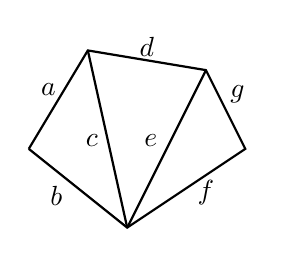
\begin{tikzpicture}
                                \draw[thick] (0.5 / 2,2 / 2) -- (2 / 2,4.5 / 2) -- (5 / 2,4 / 2) -- (6 / 2,2 / 2) -- (3 / 2,0 / 2) -- (0.5 / 2,2 / 2);
                                \draw[thick] (2 / 2,4.5 / 2) -- (3 / 2,0 / 2);
                                \draw[thick] (5 / 2,4 / 2) -- (3 / 2,0 / 2);

                                \node at (1 / 2,3.5 / 2){$a$};
                                \node at (1.2 / 2,0.8 / 2){$b$};
                                \node at (2.1 / 2,2.2 / 2){$c$};
                                \node at (3.5 / 2,4.6 / 2){$d$};
                                \node at (3.6 / 2,2.2 / 2){$e$};
                                \node at (5 / 2,0.9 / 2){$f$};
                                \node at (5.8 / 2,3.4 / 2){$g$};
                            \end{tikzpicture}
                        \end{columns}

                    \end{itemize}

                \end{exampleblock}
            }{
                \alt<2>{
                    \begin{exampleblock}{问题分析}
                        \begin{itemize}
                            \item 一个五边形可以分割为三个三角形,因此五边形的面积等于三个三角形的面积之和
                        \end{itemize}

                        \begin{columns}[onlytextwidth,T]
                            \column{.7\textwidth}
                            \begin{itemize}
                                \item 三角形的面积可以套用海伦公式求解
                            \end{itemize}

                            \column{.3\textwidth}
                            % 图像
                            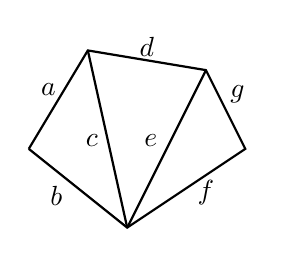
\begin{tikzpicture}
                                \draw[thick] (0.5 / 2,2 / 2) -- (2 / 2,4.5 / 2) -- (5 / 2,4 / 2) -- (6 / 2,2 / 2) -- (3 / 2,0 / 2) -- (0.5 / 2,2 / 2);
                                \draw[thick] (2 / 2,4.5 / 2) -- (3 / 2,0 / 2);
                                \draw[thick] (5 / 2,4 / 2) -- (3 / 2,0 / 2);

                                \node at (1 / 2,3.5 / 2){$a$};
                                \node at (1.2 / 2,0.8 / 2){$b$};
                                \node at (2.1 / 2,2.2 / 2){$c$};
                                \node at (3.5 / 2,4.6 / 2){$d$};
                                \node at (3.6 / 2,2.2 / 2){$e$};
                                \node at (5 / 2,0.9 / 2){$f$};
                                \node at (5.8 / 2,3.4 / 2){$g$};
                            \end{tikzpicture}
                        \end{columns}
                    \end{exampleblock}
                }{

                    \begin{exampleblock}{编程题}
                        \begin{itemize}
                            \item 如图所示的五边形,输入其 $5$ 条边和 $2$ 条对角线的边长,求这个五边形的面积。\\
                                根据海伦公式,边长分别为 $a$, $b$, $c$ 的三角形面积为 $\sqrt{p (p - a) (p - b) (p - c)}$,
                                其中 $p = \frac{a+b+c}{2}$。\\
                                输出结果保留至小数点后两位。
                        \end{itemize}

                        \begin{columns}[onlytextwidth,T]
                            \column{.7\textwidth}
                            \begin{itemize}
                                \item 样例输入
                                
                                    \lstinline|3 4 5 6 7 8 9|

                                \item 样例输出
                                
                                    \lstinline|47.53|
                            \end{itemize}
                            \column{.3\textwidth}
                                % 图像
                                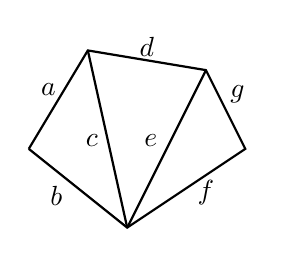
\begin{tikzpicture}
                                    \draw[thick] (0.5 / 2,2 / 2) -- (2 / 2,4.5 / 2) -- (5 / 2,4 / 2) -- (6 / 2,2 / 2) -- (3 / 2,0 / 2) -- (0.5 / 2,2 / 2);
                                    \draw[thick] (2 / 2,4.5 / 2) -- (3 / 2,0 / 2);
                                    \draw[thick] (5 / 2,4 / 2) -- (3 / 2,0 / 2);

                                    \node at (1 / 2,3.5 / 2){$a$};
                                    \node at (1.2 / 2,0.8 / 2){$b$};
                                    \node at (2.1 / 2,2.2 / 2){$c$};
                                    \node at (3.5 / 2,4.6 / 2){$d$};
                                    \node at (3.6 / 2,2.2 / 2){$e$};
                                    \node at (5 / 2,0.9 / 2){$f$};
                                    \node at (5.8 / 2,3.4 / 2){$g$};
                                \end{tikzpicture}
                        \end{columns}
                    \end{exampleblock}

                }
            }
        }
    }

\end{frame}
%------------------------------------------------------------

%------------------------------------------------------------
\begin{frame}[fragile]
    \frametitle{例 2.2:质数判断}

    \alt<7-9> {
        \begin{columns}[onlytextwidth,T]
            \column{.7\textwidth}
            \lstinputlisting[basicstyle=\ttfamily\scriptsize,language=C++,name=isPrime_2]{ch14/isPrime_2.cc}

            \begin{tikzpicture}[remember picture, overlay]
                \uncover<9>{\redbox{isPrime_2}{9}{12}{9}{12} node[right,xshift=.5cm,yshift=-0.7cm]{如果 $n$ 是 \lstinline|long long| 类型,怎么修改?};}
            \end{tikzpicture}

            \column{.3\textwidth}
            \begin{itemize}
                \item<8-> 时间复杂度 $O(\sqrt{n})$
            \end{itemize}
        \end{columns}

    } {
    \alt<6>{
        \begin{exampleblock}{质数判定的优化}
            \begin{itemize}
                \item 观察一个数字除了 $1$ 和它本身之外的因数,例如 $36$
                
                \begin{itemize}
                    \item $2, 3, 4, 6, 9, 12, 18$
                    \item 因数是成对存在的:$2 \times 18 = 36$, $3 \times 12 = 36$, ...
                \end{itemize}

                \item 成对的两个因数,其中一个 $\leq \sqrt{n}$ ,一个 $\geq \sqrt{n}$ 
                \item 如果 $n$ 不存在 $\leq \sqrt{n}$ 的因数,肯定也不存在 $\geq \sqrt{n}$ 的因数
                \item 所以判定质数代码中的 $i$ 只需要枚举到 $\sqrt{n}$ ,不用枚举到 $n - 1$
            \end{itemize}
        \end{exampleblock}
    } {
        \alt<3-5>{
            \begin{itemize}
                \item 判断 $n$ 有没有 $2 \sim n - 1$ 范围的因数
            \end{itemize}

            \only<3-4>{\lstinputlisting[basicstyle=\ttfamily\scriptsize,language=C++,name=isPrime_1]{ch14/isPrime_1.cc}}
            \only<5>{\lstinputlisting[basicstyle=\ttfamily\scriptsize,language=C++,name=isPrime_1_2]{ch14/isPrime_1_2.cc}}

            \begin{tikzpicture}[remember picture, overlay]
                \uncover<4>{\redbox{isPrime_1}{2}{3}{2}{29} node[right,xshift=.5cm,yshift=.2cm]{是否正确?};}
            \end{tikzpicture}
        } {
            \alt<2>{
                \begin{exampleblock}{质数基本概念}
                    \begin{itemize}
                        \item 整除:指整数 $a$ 除以整数 $b$ ($b \neq 0$) 的余数为 $0$ 
                        \item 因数(约数):如果 $a$ 除以 $b$ 能够整除,则 $b$ 是 $a$ 的因数(约数)
                        \item 倍数:如果 $a$ 除以 $b$ 能够整除,则 $a$ 是 $b$ 的倍数
                        \item 质数(素数):指在大于 $1$ 的自然数中,除了 $1$ 和它本身以外不再有其他因数的自然数
                    \end{itemize}
                \end{exampleblock}
            } {
                \begin{exampleblock}{编程题}
                    \begin{itemize}
                        \item 输入一个正整数 $n$ ($1 \leq n \leq 2 \times 10^9$),判断 $n$ 是否为质数。\\
                            若 $x$ 是质数,输出 \lstinline|yes|;否则输出 \lstinline|no|。
                        \item 样例输入
                                            
                            \lstinline|3|

                        \item 样例输出
                        
                            \lstinline|yes|
                
                    \end{itemize}
                \end{exampleblock}
            }
        }
    }
    }
\end{frame}
%------------------------------------------------------------

%------------------------------------------------------------
\begin{frame}[fragile]
    \frametitle{使用函数的优点}

        \begin{itemize}
            \item 将功能封装到函数中,提高代码的可读性
            \item 提高代码的复用性,使代码简洁
            \item 将代码分解成更小的块(模块化),使代码逻辑简单明了,易于查错
        \end{itemize}
    
\end{frame}
%------------------------------------------------------------

\section{局部变量和全局变量}

%------------------------------------------------------------
\begin{frame}[fragile]
    \frametitle{变量的作用域}

        \begin{itemize}
            \item 代码中的变量并不是在任何位置都可以使用
            \item 一个变量可用的代码范围就是这个变量的作用域
            \item 根据作用域的不同,可以把变量分为局部变量和全局变量
        \end{itemize}
    
\end{frame}
%------------------------------------------------------------

%------------------------------------------------------------
\begin{frame}[fragile]
    \frametitle{局部变量}

    \alt<6->{
        \begin{itemize}
            \item 函数(包含参数列表)也视作一个块
        \end{itemize}

        \lstinputlisting[basicstyle=\ttfamily\scriptsize,language=C++,name=local_var_2]{ch14/local_var_2.cc}
        \begin{tikzpicture}[remember picture, overlay]
            \uncover<7>{\redbox{local_var_2}{1}{1}{5}{39};}
        \end{tikzpicture}

        \begin{itemize}
            \item<7> 这是一个“块”,变量 \lstinline|n| 只能在这个“块”中使用
        \end{itemize}

    } {
        \alt<2-5> {
            \begin{columns}[onlytextwidth,T]
                \column{.5\textwidth}
                \lstinputlisting[basicstyle=\ttfamily\scriptsize,language=C++,name=local_var_1]{ch14/local_var_1.cc}
                \begin{tikzpicture}[remember picture, overlay]
                    \uncover<2>{\redbox{local_var_1}{3}{1}{14}{23};}
                    \uncover<3>{\redbox{local_var_1}{5}{3}{8}{13};}
                    \uncover<4>{\redbox{local_var_1}{9}{3}{11}{23};}
                    \uncover<5>{\redbox{local_var_1}{12}{3}{12}{23};}
                \end{tikzpicture}
    
                \column{.5\textwidth}
                \begin{itemize}
                    \item <2> 这是一个“块”,变量 \lstinline|n| 只能在这个“块”中使用
                    \item <3> 这是一个“块”,变量 \lstinline|a| 只能在这个“块”中使用
                    \item <4> 这是一个“块”,变量 \lstinline|i| 只能在这个“块”中使用
                    \item <5> {\textcolor{red}{编译错误:此处的 \lstinline|i| 未声明}}
                \end{itemize}
            \end{columns}
        }{
            \begin{itemize}
                \item 声明在函数内部的变量
                \item 作用域:从变量的声明开始到包含它的块结束
    
                \begin{itemize}
                    \item 块是用一对大括号括起来的代码区域
                    \item 循环、分支语句(包含条件语句)视作一个块
                    \item 函数(包含参数列表)也视作一个块
                \end{itemize}
                
            \end{itemize}
        }
    }
    
\end{frame}
%------------------------------------------------------------

%------------------------------------------------------------
\begin{frame}[fragile]
    \frametitle{全局变量}

    \alt<5-6>{
        \lstinputlisting[basicstyle=\ttfamily\scriptsize,language=C++,name=global_var_2]{ch14/global_var_2.cc}
        \begin{tikzpicture}[remember picture, overlay]
            \uncover<6>{\redbox{global_var_2}{14}{1}{15}{36};}
        \end{tikzpicture}

        \begin{itemize}
            \item<6> 能成功编译吗?
        \end{itemize}
    } {
        \alt<2-4> {
            \begin{columns}[onlytextwidth,T]
                \column{.6\textwidth}
                \lstinputlisting[basicstyle=\ttfamily\scriptsize,language=C++,name=global_var_1]{ch14/global_var_1.cc}
                \begin{tikzpicture}[remember picture, overlay]
                    \uncover<2>{\redbox{global_var_1}{11}{1}{11}{36};}
                    \uncover<3>{\redbox{global_var_1}{12}{1}{12}{36};}
                    \uncover<4>{\redbox{global_var_1}{13}{1}{13}{36};}
                \end{tikzpicture}

                \column{.4\textwidth}
                \begin{itemize}
                    \item 输出\\
                    
                        \uncover<3->{\lstinline|main(): 1|\\}
                        \uncover<4->{\lstinline|f(): 1|}

                \end{itemize}
            \end{columns}
        } {
            \begin{itemize}
                \item 定义在所有函数外部、没有被任何大括号包含起来的变量
                \item 作用域:从变量的声明开始一直到代码结束,作用域中任意的函数都可以使用该变量
            \end{itemize}
        }
    }
        
\end{frame}
%------------------------------------------------------------

\section{同名变量和引用变量}

%------------------------------------------------------------
\begin{frame}[fragile]
    \frametitle{同名变量}

    \alt<9> {
        \begin{itemize}
            \item 函数:输出 $1 \sim n$ 的和
        \end{itemize}
        \lstinputlisting[basicstyle=\ttfamily\scriptsize,language=C++,name=get_sum]{ch14/get_sum.cc}
        \begin{tikzpicture}[remember picture, overlay]
            \uncover<9>{\redbox{get_sum}{3}{12}{3}{16};}
            \uncover<9>{\redbox{get_sum}{12}{3}{12}{7};}
        \end{tikzpicture}
    } {
    \alt<8> {
        \begin{itemize}
            \item 函数:输出 $n$ 行 \lstinline|hello world|
        \end{itemize}
        \lstinputlisting[basicstyle=\ttfamily\scriptsize,language=C++,name=say_hello]{ch14/say_hello.cc}
        \begin{tikzpicture}[remember picture, overlay]
            \uncover<8>{\redbox{say_hello}{5}{15}{5}{19};}
            \uncover<8>{\redbox{say_hello}{12}{3}{12}{7};}
        \end{tikzpicture}
    } {
        \alt<6-7> {
            \begin{itemize}
                \item 查询第一个 \lstinline|x| 所在位置
            \end{itemize}

            \lstinputlisting[basicstyle=\ttfamily\scriptsize,language=C++,name=search_x]{ch14/search_x.cc}
                \begin{tikzpicture}[remember picture, overlay]
                    \uncover<6->{\redbox{search_x}{10}{3}{10}{44};}
                    \uncover<7>{\redbox{search_x}{13}{3}{18}{32} node[below, xshift=0cm, yshift=0cm]{两个“块”完全不重叠, 变量 \lstinline|i| 互不影响};}
                \end{tikzpicture}
        } {
            \alt<2-5> {
                \begin{itemize}
                    \item 输出 $3$ 行 $4$ 列的星号 \lstinline|*|
                \end{itemize}

                \lstinputlisting[basicstyle=\ttfamily\scriptsize,language=C++,name=star]{ch14/star.cc}
                \begin{tikzpicture}[remember picture, overlay]
                    \uncover<3->{\redbox{star}{1}{1}{6}{33};}
                    \uncover<4->{\redbox{star}{2}{3}{4}{32};}
                \end{tikzpicture}

                \begin{itemize}
                    \item<4-> 第一层 \lstinline|for| 循环完全覆盖第二层 \lstinline|for| 循环
                    \item<5-> \lstinline|i| 的声明屏蔽了外部的 \lstinline|i|, 若此时使用 \lstinline|i|, 
                            则使用的是内部的 \lstinline|i| 容易混淆两个 \lstinline|i| 的使用
                \end{itemize}
            } {
                \begin{itemize}
                    \item 在同一个“块”里面声明的同名变量冲突
                    \item 在不同“块” 里面声明的同名变量不冲突

                    \begin{itemize}
                        \item 完全覆盖
                        \item 完全不覆盖
                    \end{itemize}
                    
                \end{itemize}
            }
        }
    }
    }
    
\end{frame}
%------------------------------------------------------------

%------------------------------------------------------------
\begin{frame}[fragile]
    \frametitle{引用变量}

    \alt<4-9> {
        \begin{columns}[onlytextwidth,T]
            \column{.5\textwidth}
            \lstinputlisting[basicstyle=\ttfamily\scriptsize,language=C++,name=refer_var]{ch14/refer_var.cc}
            \begin{tikzpicture}[remember picture, overlay]
                \uncover<5>{\redbox{refer_var}{6}{3}{6}{20};}
                \uncover<6>{\redbox{refer_var}{7}{3}{7}{20};}
                \uncover<7>{\redbox{refer_var}{8}{3}{8}{20};}
                \uncover<8>{\redbox{refer_var}{9}{3}{9}{20};}
                \uncover<9>{\redbox{refer_var}{10}{3}{10}{20};}
            \end{tikzpicture}

            \column{.5\textwidth}
            \begin{itemize}
                \item 内存
            \end{itemize}

            \begin{tikzpicture}
                [nodes in empty cells, nodes={minimum width=1cm, minimum height=.7cm}, row sep=-\pgflinewidth, column sep=-\pgflinewidth]

                \only<4>{
                    \matrix(A) [matrix of nodes, ampersand replacement=\&, row 1/.style={nodes={draw=none}}, nodes={draw, anchor=center}]{
                        \\
                        \lstinline|...| \& \& \& \& \lstinline|...| \\
                    };
                }
                \only<5>{
                    \matrix(A) [matrix of nodes, ampersand replacement=\&, row 1/.style={nodes={draw=none}}, nodes={draw, anchor=center}]{
                        \\
                        \lstinline|...|   \& \& \lstinline|1|   \& \& \lstinline|...| \\
                    };
                    \node (x) [rectangle, minimum height=.5cm, text centered, text width=2cm, draw=black, font=\footnotesize, below of=A, yshift=-.5cm] {我的名字是 \lstinline|x|};
                    \draw [arrow] (x) -- (A);
                }
                \only<6>{
                    \matrix(A) [matrix of nodes, ampersand replacement=\&, row 1/.style={nodes={draw=none}}, nodes={draw, anchor=center}]{
                        \\
                        \lstinline|...|   \& \& \lstinline|1|   \& \& \lstinline|...| \\
                    };
                    \node (x) [rectangle, minimum height=.5cm, text centered, text width=2cm, draw=black, font=\footnotesize, below of=A, xshift=-1.5cm, yshift=-.5cm] {我的名字是 \lstinline|x|};
                    \node (y) [rectangle, minimum height=.5cm, text centered, text width=2.5cm, draw=black, font=\footnotesize, below of=A, xshift=1.5cm, yshift=-.5cm] {我多了个名字 \lstinline|y|};
                    \draw [arrow] (x) -- (A.south);
                    \draw [arrow] (y) -- (A.south);
                }
                \only<7-9>{
                    \matrix(A) [matrix of nodes, ampersand replacement=\&, row 1/.style={nodes={draw=none}}, nodes={draw, anchor=center}]{
                        \\
                        \lstinline|...|   \& \& \lstinline|2|   \& \& \lstinline|...| \\
                    };
                    \node (x) [rectangle, minimum height=.5cm, text centered, text width=2cm, draw=black, font=\footnotesize, below of=A, xshift=-1.5cm, yshift=-.5cm] {我的名字是 \lstinline|x|};
                    \node (y) [rectangle, minimum height=.5cm, text centered, text width=2.5cm, draw=black, font=\footnotesize, below of=A, xshift=1.5cm, yshift=-.5cm] {我多了个名字 \lstinline|y|};
                    \draw [arrow] (x) -- (A.south);
                    \draw [arrow] (y) -- (A.south);
                }
                
            \end{tikzpicture}

            \begin{itemize}
                \item<8-> 输出\\
                    \uncover<8->{\lstinline|2|\\}
                    \uncover<9->{\lstinline|2|}
            \end{itemize}

        \end{columns}
    } {
        \alt<2-3>{
            \begin{itemize}
                \item<2-> 一般变量

                \begin{itemize}
                    \item 一般变量在声明时,会被分配一个独立的内存空间
                \end{itemize}
                
                \item<3-> 引用变量

                \begin{itemize}
                    \item 引用变量是其他变量的别名,与其他变量共用同一块内存空间
                    \item 在变量类型和变量名之间加一个 \lstinline|&|,表示该变量是一个引用

                    \begin{itemize}
                        \item \textbf{数据类型 \textcolor{red}{\lstinline|&|} 引用变量名 \lstinline|=| 被引用的变量名;}
                        \item 引用需要在声明的时候进行初始化,与一个固定的变量绑定
                    \end{itemize}

                \end{itemize}
                
            \end{itemize}    
        }{
            \begin{block}{}
                \vspace{.5cm}
                \begin{center}
                    两个变量可以用相同名称,\\
                    那么同一个变量可不可以有不同名称?
                \end{center}
                \vspace{.5cm}
            \end{block}
        }
    }
    
\end{frame}
%------------------------------------------------------------

%------------------------------------------------------------
\begin{frame}[fragile]
    \frametitle{交换变量的值}

    \alt<2-7>{
        \begin{columns}[onlytextwidth,T]
            \column{.5\textwidth}
            \lstinputlisting[basicstyle=\ttfamily\scriptsize,language=C++,name=my_swap_1]{ch14/my_swap_1.cc}
            \begin{tikzpicture}[remember picture, overlay]
                \uncover<3>{\redbox{my_swap_1}{10}{3}{10}{28};}
                \uncover<4-6>{\redbox{my_swap_1}{11}{3}{11}{28};}
                \uncover<5>{\redbox{my_swap_1}{3}{1}{3}{28};}
                \uncover<6>{\redbox{my_swap_1}{4}{3}{6}{28};}
                \uncover<7>{\redbox{my_swap_1}{12}{3}{12}{33};}
            \end{tikzpicture}

            \column{.5\textwidth}
            \begin{itemize}
                \item 内存
            \end{itemize}

            \begin{tikzpicture}
                [nodes in empty cells, nodes={minimum width=0.8cm, minimum height=.7cm}, row sep=-\pgflinewidth, column sep=-\pgflinewidth]

                \only<2>{
                    \matrix(A) [matrix of nodes, ampersand replacement=\&, row 1/.style={nodes={draw=none}}, nodes={draw, anchor=center}]{
                        \\
                        \lstinline|...| \& \& \& \lstinline|...| \& \& \& \lstinline|...| \\
                    };
                }
                \only<3-4>{
                    \matrix(A) [matrix of nodes, ampersand replacement=\&, row 1/.style={nodes={draw=none}}, nodes={draw, anchor=center}]{
                                        \& \lstinline|x|\& \lstinline|y| \\
                        \lstinline|...| \& \lstinline|1|\& \lstinline|2| \& \lstinline|...| \& \& \& \lstinline|...| \\
                    };
                }
                \only<5>{
                    \matrix(A) [matrix of nodes, ampersand replacement=\&, row 1/.style={nodes={draw=none}}, nodes={draw, anchor=center}]{
                                        \& \lstinline|x|\& \lstinline|y| \&                 \& \lstinline|a| \& \lstinline|b| \\
                        \lstinline|...| \& \lstinline|1|\& \lstinline|2| \& \lstinline|...| \& \lstinline|1| \& \lstinline|2| \& \lstinline|...| \\
                    };
                }
                \only<6>{
                    \matrix(A) [matrix of nodes, ampersand replacement=\&, row 1/.style={nodes={draw=none}}, nodes={draw, anchor=center}]{
                                        \& \lstinline|x|\& \lstinline|y| \&                 \& \lstinline|a| \& \lstinline|b| \\
                        \lstinline|...| \& \lstinline|1|\& \lstinline|2| \& \lstinline|...| \& \lstinline|2| \& \lstinline|1| \& \lstinline|...| \\
                    };
                }
                \only<7>{
                    \matrix(A) [matrix of nodes, ampersand replacement=\&, row 1/.style={nodes={draw=none}}, nodes={draw, anchor=center}]{
                                        \& \lstinline|x|\& \lstinline|y| \& \& \& \\
                        \lstinline|...| \& \lstinline|1|\& \lstinline|2| \& \lstinline|...| \& \lstinline|2| \& \lstinline|1| \& \lstinline|...| \\
                    };
                }
            \end{tikzpicture}

            \begin{itemize}
                \item<7> 输出\\
                    \uncover<7>{\lstinline|1 2|}
            \end{itemize}

        \end{columns}
    }{
        \begin{block}{}
            \vspace{.5cm}
            \begin{center}   
                交换两个变量的值,如何用函数实现?
            \end{center}
            \vspace{.5cm}
        \end{block}
    }
\end{frame}
%------------------------------------------------------------

%------------------------------------------------------------
\begin{frame}[fragile]
    \frametitle{参数传递}

    \alt<8->{
        \begin{itemize}
            \item 按值传递

            \begin{itemize}
                \item 传递的是数值,形参与实参是不同变量,修改形参不影响实参
                \item 不需要在函数中修改实参时使用
            \end{itemize}
            
            \item 按引用传递

            \begin{itemize}
                \item 传递变量本身,形参与实参是同一个变量
                \item 需要在函数中修改实参时使用
            \end{itemize}
            
        \end{itemize}
    }{
        \alt<2-7>{
            \begin{columns}[onlytextwidth,T]
                \column{.6\textwidth}
                \lstinputlisting[basicstyle=\ttfamily\scriptsize,language=C++,name=my_swap_2]{ch14/my_swap_2.cc}
                \begin{tikzpicture}[remember picture, overlay]
                    \uncover<3>{\redbox{my_swap_2}{10}{3}{10}{27};}
                    \uncover<4-6>{\redbox{my_swap_2}{11}{3}{11}{15};}
                    \uncover<5>{\redbox{my_swap_2}{3}{1}{3}{27};}
                    \uncover<5>{\draw[red, very thick, ->] ([shift={(2pt, .25em)}] pic cs:line-my_swap_2-11-end) -- ++(8em, 0) |- node[left,yshift=-1.5cm,text width=2cm] {\lstinline|int &a = x; int &b = y;|}([shift={(2pt, .25em)}] pic cs:line-my_swap_2-3-end);}
                    \uncover<6>{\redbox{my_swap_2}{4}{3}{6}{15};}
                    \uncover<7>{\redbox{my_swap_2}{12}{3}{12}{33};}
                \end{tikzpicture}

                \column{.4\textwidth}
                \begin{itemize}
                    \item 内存
                \end{itemize}

                \begin{tikzpicture}
                    [nodes in empty cells, nodes={minimum width=0.8cm, minimum height=.7cm}, row sep=-\pgflinewidth, column sep=-\pgflinewidth]

                    \only<2>{
                        \matrix(A) [matrix of nodes, ampersand replacement=\&, row 1/.style={nodes={draw=none}}, nodes={draw, anchor=center}]{
                            \\
                            \lstinline|...| \& \& \& \lstinline|...| \\
                        };
                    }
                    \only<3-4>{
                        \matrix(A) [matrix of nodes, ampersand replacement=\&, row 1/.style={nodes={draw=none}}, nodes={draw, anchor=center}]{
                                            \& \lstinline|x|\& \lstinline|y| \\
                            \lstinline|...| \& \lstinline|1|\& \lstinline|2| \& \lstinline|...| \\
                        };
                    }
                    \only<5>{
                        \matrix(A) [matrix of nodes, ampersand replacement=\&, row 1/.style={nodes={draw=none}}, nodes={draw, anchor=center}]{
                                            \& \lstinline|x|\& \lstinline|y| \\
                            \lstinline|...| \& \lstinline|1|\& \lstinline|2| \& \lstinline|...| \\
                        };
                        \node (a) [rectangle, minimum height=.5cm, text centered, text width=0.7cm, draw=white, font=\footnotesize, below of=A, xshift=-.4cm] {\textcolor{black}{\lstinline|a|}};
                        \node (b) [rectangle, minimum height=.5cm, text centered, text width=0.7cm, draw=white, font=\footnotesize, below of=A, xshift=.4cm] {\textcolor{black}{\lstinline|b|}};
                    }
                    \only<6-7>{
                        \matrix(A) [matrix of nodes, ampersand replacement=\&, row 1/.style={nodes={draw=none}}, nodes={draw, anchor=center}]{
                                            \& \lstinline|x|\& \lstinline|y| \\
                            \lstinline|...| \& \lstinline|2|\& \lstinline|1| \& \lstinline|...| \\
                        };
                        \node (a) [rectangle, minimum height=.5cm, text centered, text width=0.7cm, draw=white, font=\footnotesize, below of=A, xshift=-.4cm] {\textcolor{black}{\lstinline|a|}};
                        \node (b) [rectangle, minimum height=.5cm, text centered, text width=0.7cm, draw=white, font=\footnotesize, below of=A, xshift=.4cm] {\textcolor{black}{\lstinline|b|}};
                    }
                    
                \end{tikzpicture}

                \begin{itemize}
                    \item<7> 输出\\
                        \uncover<7>{\lstinline|2 1|}
                \end{itemize}

            \end{columns}
        }{
            \begin{itemize}
                \item 按值传递

                \begin{itemize}
                    \item 若参数声明为一般形式,参数传递时只是将实参的数值赋值给形参,函数不能访问实参本身
                \end{itemize}
                
                \item 按引用传递

                \begin{itemize}
                    \item 引用变量是其他变量的别名,与其他变量共用同一块内存空间
                    \item 将形式参数声明为引用类型,可以访问和修改实参本身
                \end{itemize}
                
            \end{itemize}
        }
    }
        
\end{frame}
%------------------------------------------------------------

\section{数组参数传递}

%------------------------------------------------------------
\begin{frame}[fragile]
    \frametitle{数组参数传递}

    \alt<5->{
        \begin{itemize}
            \item 数组储存在一块连续的内存中
            \item<6-> 内存中每个位置有个“编号”,即“内存地址”
            
            \begin{itemize}
                \item<5-> 通过数组名 \lstinline|a| 可以访问到这个数组的首地址
            \end{itemize}

        \end{itemize}

        \begin{tikzpicture}
            [nodes in empty cells, nodes={minimum width=0.8cm, minimum height=.7cm}, row sep=-\pgflinewidth, column sep=-\pgflinewidth]
            \only<5-6>{
                \matrix(A) [matrix of nodes, ampersand replacement=\&, row 1/.style={nodes={draw=none}}, nodes={draw, anchor=center}]{
                    \\
                    \lstinline|...| \& \lstinline|a[0]| \& \lstinline|a[1]| \& \lstinline|a[2]| \& \lstinline|a[3]| \& \lstinline|...| \\
                };
            }
            \uncover<7->{
                \matrix(A) [matrix of nodes, ampersand replacement=\&, row 1/.style={nodes={draw=none}}, nodes={draw, anchor=center}]{
                    \\
                    \lstinline|...| \& \textcolor{red}{\lstinline|a[0]|} \& \lstinline|a[1]| \& \lstinline|a[2]| \& \lstinline|a[3]| \& \lstinline|...| \\
                };
                \node (a) [rectangle, minimum height=.5cm, text centered, text width=7cm, draw=white, font=\footnotesize, above of=A, xshift=.5cm, yshift=-.5cm] {\textcolor{black}{输出数组名 \lstinline|a| 可以看到这块内存的“编号”}};
            }
        \end{tikzpicture}

        \begin{itemize}   
            \item<6-> 数组元素是通过首地址 + 偏移量来访问的
            
            \begin{itemize}
                \item<6-> \lstinline|a[1]| 储存在首地址往后偏移 $1$ 个位置,\lstinline|a[2]| 储存在首地址往后偏移 $2$ 个位置……
            \end{itemize}

        \end{itemize}
    }{
        \alt<2-4>{
            \begin{itemize}
                \item<2-> 按值传递?

                \begin{itemize}
                    \item<3-> 把实参数组所有元素复制到形参数组中,需要付出的时间和储存空间代价过大
                    \item<3-> C++ 不支持按值传递数组
                \end{itemize}
                
                \item<4> 函数传递数组默认用类似按引用传递的方式

                \begin{itemize}
                    \item 形参格式:\textbf{数据类型\quad 数组名[]}
                    \item 不需要使用引用传递
                \end{itemize}
                
            \end{itemize}
        }{
            \begin{block}{}
                \vspace{.5cm}
                \begin{center}   
                    参数是数组,应该按什么方式传递?
                \end{center}
                \vspace{.5cm}
            \end{block}
        }
    }
    
\end{frame}
%------------------------------------------------------------

%------------------------------------------------------------
\begin{frame}[fragile]
    \frametitle{首地址与参数传递}
    \begin{itemize}
        \item 只要知道数组的首地址,就能访问到数组的每个元素
        \item 参数传递首地址,被调用的函数就能访问原数组
        
        \begin{itemize}
            \item 传递的是地址,效果类似按引用传递
            \item 数组名的值表示数组首地址,实参填写数组名即可
        \end{itemize}
        
    \end{itemize}

\end{frame}
%------------------------------------------------------------

%------------------------------------------------------------
\begin{frame}[fragile]
    \frametitle{例 2.3:一维数组的输入输出}

    \alt<2-4> {
        \lstinputlisting[basicstyle=\ttfamily\scriptsize,language=C++,name=arr_io]{ch14/arr_io.cc}

        \begin{tikzpicture}[remember picture, overlay]
            \uncover<3->{\redbox{arr_io}{4}{12}{4}{18} node[right,xshift=1.7cm,yshift=.3cm]{形参加 \lstinline|[]|};}
            \uncover<4>{\redbox{arr_io}{19}{3}{20}{15} node[right,xshift=.3cm,yshift=.5cm]{注意实参写数组名即可,不能写成 \lstinline|A[110]|};}
        \end{tikzpicture}

    } {
        \begin{exampleblock}{编程题}
            \begin{itemize}
                \item 实现一个 \lstinline|input| 函数,功能:将 $n$ 个整数存入一维数组中;\\
                    实现一个 \lstinline|output| 函数,功能:顺序输出数组中的 $n$ 个整数,数字之间以空格间隔。\\
                    请调用上述函数,输入 $n$ ($n \le 100$) 个整数,顺序输出这 $n$ 个整数。\\
                \item 样例输入

                    \lstinline|5|\\
                    \lstinline|3 1 5 2 8|

                \item 样例输出
                
                    \lstinline|3 1 5 2 8|

            \end{itemize}
        \end{exampleblock}
    }

\end{frame}
%------------------------------------------------------------

%------------------------------------------------------------
\begin{frame}[fragile]
    \frametitle{小结:参数传递}

    \begin{itemize}
        \item<1-> 按值传递(被调用的函数不会影响实参)
        
        \begin{itemize}
            \item 形参的声明:和声明普通变量一样
        \end{itemize}

        \item<2-> 按引用传递(被调用的函数能修改实参的值)
        
        \begin{itemize}
            \item 形参的声明:变量名前面加 \lstinline|&|
        \end{itemize}

        \item<3-> 数组传递(传递首地址,效果类似按引用传递)
        
        \begin{itemize}
            \item 形参的声明:数组名后面加 \lstinline|[]|
        \end{itemize}

    \end{itemize}

\end{frame}
%------------------------------------------------------------


\section{总结}

% ------------------------------------------------------------
\begin{frame}[fragile]
    \frametitle{总结}
    \begin{itemize}
        \item<1-> 函数的设计
        
        \begin{itemize}
            \item 模块化编程
            \item 函数的优点和适用场景
        \end{itemize}

        \item<2-> 变量
        
        \begin{itemize}
            \item 作用域
            \item 同名变量
            \item 引用变量
        \end{itemize}

        \item<3-> 函数参数传递
        
        \begin{itemize}
            \item 按值传递
            \item 按引用传递
            \item 数组传递
        \end{itemize}

    \end{itemize}
\end{frame}
%------------------------------------------------------------

\end{document}
